\chapter{Concept}\label{chap:Concept}

\section{The type system}\label{sec:concept:TheTypeSystem}

In \ref{subsec:background:TypeSystems}, we introduce the concept of type systems and we give a brief overview of \textit{type checking} and \textit{type inference}. Our goal is to have solid \textit{application programming interfaces} (APIs) to build type systems for each language.

In this section, we will discuss the importance of the type system for our concept.
What we are looking for in our type system is:
\begin{itemize}
    \item \textbf{modularization}, that allows the definition of custom types and operations on these types, and the ability to combine them in a modular way;
    \item \textbf{flexibility}, since the type system is not known \textit{a priori}, we need the ability to adapt the type system to the specific needs;
    \item \textbf{easy-to-use}, extending the default implementation of the type system with a new type, or implementing a new type from scratch should be easy and straightforward.
\end{itemize}

It is trivial to remember that the type system should also provide the basic functionalities of a type system, such as \textbf{type inference}, that allows the compiler to infer the type of an expression without the need to explicitly specify it; and \textbf{type checking}, that allows the compiler to check if the types of the expressions are correct.


\begin{mydefinition}{Type system item}{concept:itemdefinition}
  % This is the text of the theorem. The counter is automatically assigned and,
  % in this example, prefixed with the section number. This theorem is numbered with
  %   \ref{def:concept:itemdefinition} and is given on page \pageref{def:concept:itemdefinition}.
    Given that the specifics of the target language for the reference type system are not predetermined (i.e., the language is not known \textit{a priori}), we cannot assume the presence of standard programming constructs such as variables, functions, or objects. Therefore, to maintain a broad and adaptable approach, we will use the term \textbf{item} to refer to any of these potential constructs or elements within the system. This ensures that our discussion remains relevant regardless of the particular features and paradigms of the target language.
\end{mydefinition}

\subsection{Type: the basic building block}\label{subsec:concept:TypeTheBasicBuildingBlock}

The \textbf{Type} is the basic building block of the type system. It is used to represent the type of an expression, such as a variable, a function, or an object. The \textbf{Type} can be a primitive type, such as \textit{int}, \textit{float}, \textit{string} or a custom type, such as a \textit{class}, \textit{interface}, or \textit{enum}.

\begin{mydefinition}{Type}{concept:type}
The name \textbf{type} could be misleading because it does not exactly represent the type of an item but rather it is class of types that allows to build a specific type of a given category. Note that, this is not excluing that each concreate type could have a specific (class of) \textbf{type}, but defining a \textbf{type} as a class of types allows to define a generic \textbf{type} for all the types of a given category (i.e., all primitive types) and defining once the operations that can be performed on them.
\end{mydefinition}

In our concept, during the implementation of the type system, several types will be defined. Each type will have a set of operations that can be performed on it. In abstract terms, we can define a type as a set of operations that can be performed on it.
Basically, each type should be answer to the following questions:
\begin{enumerate}
    \item What is its \textbf{identifier}?
    \item Can it be \textbf{assignable from} another type with a specific kind of \textbf{variance}?
    \item Can it match a specific \textbf{signature}?
    \item Does it need other types to be \textbf{bound}?
\end{enumerate}

The second question is used to \textbf{type check} the \textit{item} in the \textbf{Type System}. The type of \textbf{variance} is used to define the relationship between two types. The variance can be \textit{covariant}, \textit{contravariant}, or \textit{invariant}.

\begin{definition}{Variance}\\
    Suppose $A$ and $B$ are types, and $I[U]$ denotes application of a type constructor I with type argument $U$. Within the type system of a programming language, a typing rule for a type constructor $I$ is:
    \begin{itemize}
        \item covariant if it preserves the ordering of types ($\leq$), which orders types from more specific to more generic: If $A \leq B$, then $I[A] \leq I[B]$;
        \item contravariant if it reverses this ordering: If $A \leq B$, then $I[B] \leq I[A]$;
        \item bivariant if both of these apply (i.e., if $A \leq B$, then $I[A] \equiv I[B]$);
        \item variant if covariant, contravariant or bivariant;
        \item invariant or nonvariant if not variant.
    \end{itemize}
\end{definition}

The third question is used to \textbf{type inference} the \textit{item} in the \textbf{Type System}, simply answering to the question: can the type of the \textit{item} match a specific \textbf{signature}?
Finally, the last question is used to \textbf{bind} the type to its generic parameters. For example, the type \textit{List<String>} is bound to the type \textit{List<T>} with \textit{needed types} being \textit{String}.


\subsection{Scope: the context of the type}\label{subsec:concept:ScopeTheContextOfTheType}

\begin{mydefinition}{Scope}{concept:scope}
The \textbf{Scope} is the context in which an identifier is defined, more precisely, where the binding between the type and an identifier is defined in the \textbf{Type System}. It is used to define the visibility and the lifetime of the identifier and its operations. The \textbf{Scope} can be, for example, a \textit{local scope}, a \textit{global scope}, or a \textit{module scope}.
\end{mydefinition}

In our concept, a \textbf{Scope} can be see as a \textbf{Type}~\ref{subsec:concept:TypeTheBasicBuildingBlock} that defines the visibility and the lifetime of the type or identifier and its operations. At this point, the \textbf{Scope} is not universal. In fact, for instance, \textit{Java} do not categorize the \textbf{Scope}, such as \textit{Block Scope}, as a \textbf{Type}. However, in order to achieve a representation of a \textit{Block Scope} as a \textbf{Type}, we can define a \textbf{Scope} where at the questions

\begin{itemize}
    \item Can it be assignable from another type with a specific kind of variance?
    \item Can it match a specific signature?
\end{itemize}

will answer \textit{false}.

So, a \textbf{Scope} should be able to answer to the following questions, in addition to the questions that a \textbf{Type} should be able to answer:

\begin{enumerate}
    \item What types are \textbf{visible} in the \textbf{Scope}?
    \item Can a type be bound to an identifier in the \textbf{Scope}?
    \item If exists, what is the \textbf{parent Scope}?
    \item Can a \textbf{Scope} be marked as \textbf{external visible} and what items exported?
\end{enumerate}

The first question is used to define the visibility of the type in the \textbf{Scope} and knowing what types are visible in the \textbf{Scope}.~\ref{subsec:concept:TypingEnvironmentTheSymbolTable} will be used to answer this question.
The second question is used to bind a type to the Scope. Every scope should have a set of rules that allow to determine if a type can be bound to the Scope.~\ref{subsubsec:concept:EntryTypeBinderAnHelperToBindTypes} will be used to answer this question.
The third question is used to define the hierarchy of the Scopes. Trivially, this is represented as a tree.
Finally, the last question is used to define the visibility of the Scope and its items. A \textbf{Scope} marked as \textit{external visible} should be able to export some its items. This is useful during \textit{type inference} phase, because whan searching for a type if a Scope (type) is marked as \textit{external visible} the search should be performed recursively in all \textbf{items} exported by the \textbf{Scope}.

Now, we propose some examples of scopes in the world of object-oriented programming (OOP) languages.
In OOP there are several types of scopes that determine the visibility and lifetime of items. The most common scopes are:
\begin{itemize}
    \item \textbf{Class scope}:  A class is a collection of variables and methods. Variables declared inside a class have class scope, and they can be accessed within that class and its instances. Methods declared inside a class also have class scope and can be accessed within that class and its instances.
    \item \textbf{Instance scope}: An instance is an object created from a class. Instance variables are declared inside a class, but outside any method, and have instance scope. They can be accessed within that class’s methods and any instance of that class.
    \item \textbf{Method scope}: Variables declared inside a method have method scope, and they can only be accessed within that method.
    \item \textbf{Block scope}: A block is a section of code enclosed in curly braces. Variables declared inside a block have block scope, and they can only be accessed within that block. This includes loops, conditional statements, and code enclosed in curly braces.
    \item \textbf{Static scope}: Static variables and methods belong to a class, not to an instance of that class. Static variables and methods have class scope and can be accessed using the class name without creating an instance of the class.
\end{itemize}

\subsection{Signature: the definition of the type}\label{subsec:concept:SignatureTheDefinitionOfTheType}

A \textbf{Signature} is the definition of the type. It is used to define the structure of the type and to support \textit{static typing} and \textit{type checking}. In our type system, \textbf{each type} should have a Signature that defines the structure of the type.

\begin{mydefinition}{Signature}{concept:signature}
    The \textbf{Signature} in \textbf{structural type system}~\cite{Cardelli88, Cook89} or in \textbf{nominal type system}~\cite{Pierce02} is the definition of the type. In a \textbf{structural type system}, the \textbf{Signature} is the structure of the type, while in a \textbf{nominal type system}, the \textbf{Signature} is the name of the type. The \textbf{Signature} is used also to support \textit{static typing} and \textit{type checking}.
\end{mydefinition}

A \textbf{structural type system} is a major class of type systems in which type compatibility and equivalence are determined by the type's actual structure or definition and not by other characteristics such as its name or place of declaration. A type system is \textbf{nominal} if compatibility and equivalence of data types is determined by explicit declarations and/or the name of the types.

A \textbf{Signature} should be able to answer to one question:

\begin{enumerate}
    \item Can a type match the \textbf{Signature}?
    \item Can I resolve the type of an identifier from the \textbf{Signature}?
\end{enumerate}

Answering to this question can be simple or complex, depending on the type we would like to match with the \textbf{Signature}. For example, a type can be a primitive type, such as \textit{int}, \textit{float}, \textit{string}, or a custom type, such as a \textit{method} inside a \textit{class}.
For instance, a \textbf{Signature} is often used to define the type of a function. In this case, the \textbf{Signature} is the definition of the function in terms of its parameters and return type.
Usually, every \texttt{Type} should have a \texttt{Signature} that defines the structure of the type.
Additionally, to perform \textit{type inference}, the \textbf{Signature} is used to infer the type of an expression.

\subsection{Symbol Table Entry: an entry in the Typing Environment}\label{subsec:concept:SymbolTableEntryAnEntryInTheTypingEnvironment}

A \textbf{Symbol Table Entry} is an entry in the \textbf{Typing Environment} (Symbol Table). It is used to store a informations associated to a symbol in the \textbf{Type System}.

\begin{mydefinition}{Symbol}{concept:symbol}
    A \textbf{Symbol} is a name that represents a value, a variable, a function, or any other item in a program. In the \textbf{Type System}, a \textbf{Symbol} is used to represent a type, a variable, a function, or any other item in the program.
    Usually, symbols are collected during the \textit{parsing} phase of the compilation process and stored in a \textbf{Symbol Table}.
    A symbol can be a \textit{nonterminal symbol} or a \textit{terminal symbol}. A \textit{nonterminal symbol} is a symbol that can be expanded into other symbols, while a \textit{terminal symbol} is a symbol that cannot be expanded further.
\end{mydefinition}


The \textbf{Symbol Table Entry} should be able to answer, at least, to the following questions:
\begin{enumerate}
    \item What is the \textbf{Type} of of the associated symbol?
    \item What is the \textbf{Kind} of of the associated symbol?
    \item What is the \textbf{Location} of of the associated symbol?
    \item What are the \textbf{Details} of of the associated symbol?
\end{enumerate}

As one can guess, the \textbf{Symbol Table Entry} is used to store the information associated with a symbol in the \textbf{Type System}.
Note that to answer the first question, the \textbf{Symbol Table Entry} should have a \textbf{Type} associated with it. The answer to the second question of~\ref{subsec:concept:SignatureTheDefinitionOfTheType} can help to infer the \textbf{Type} of the associated symbol if the \textbf{Type} is not explicitly defined.
The second question is used to define the \textbf{Kind} of the associated symbol. The \textbf{Kind} can be, for example, a \textit{declaration}, a \textit{definition}, a \textit{use} or an \textit{import}.
The third question is used to define the \textbf{Location} of the associated symbol. The \textbf{Location} can be, for example, a \textit{line number} or a \textit{column number}.
Finally, the last question is used to define the \textbf{Details} of the associated symbol. The \textbf{Details} can be, for example, a \textit{description} or \textit{extra information} about the symbol.

\subsubsection{Entry Type Binder: an helper to perform type binding}\label{subsubsec:concept:EntryTypeBinderAnHelperToBindTypes}

The \textbf{Entry Type Binder} is an helper to perform type binding in the \textbf{Type System}. It is used to bind a type to an identifier in the \textbf{Scope}.
The \textbf{Entry Type Binder} should be able to answer to the following questions:
\begin{enumerate}
    \item Is this identifier already bound to the \textbf{Scope}?
    \item Can I bind an identifier to a \texttt{SymbolTableEntry} in this \textbf{Scope}?
\end{enumerate}

The first question is used to determine if the identifier is already bound to the \textbf{Scope}. If the identifier is already bound to the \textbf{Scope}, the \textbf{Entry Type Binder} should return an error.
The second question is used to determine if the identifier can be bound to a \texttt{SymbolTableEntry} in the \textbf{Scope}. If the identifier can be bound to a \texttt{SymbolTableEntry} in the \textbf{Scope}, the \textbf{Entry Type Binder} should bind the identifier to the \texttt{SymbolTableEntry}.

\subsection{Typing Environment: the symbol table}\label{subsec:concept:TypingEnvironmentTheSymbolTable}

The \textbf{Typing Environment} is the symbol table in the \textbf{Type System}. It is used to store the information associated with the symbols in the \textbf{Type System}.
Basically, the \textbf{Typing Environment} is a map between symbol or identifier and \texttt{SymbolTableEntry}.

The \textbf{Typing Environment} should be able to answer to the following questions:
\begin{enumerate}
    \item What are the symbols in the \textbf{Typing Environment}?
    \item Can I get the \texttt{SymbolTableEntry} associated with a symbol in the \textbf{Typing Environment}?
    \item Can I add a symbol to the \textbf{Typing Environment}?
    \item Can I remove a symbol from the \textbf{Typing Environment}?
\end{enumerate}

In section~\ref{subsec:concept:ScopeTheContextOfTheType}, we defined the \textbf{Scope}. Combining the \textbf{Scope} with the \textbf{Typing Environment}, we can define the visibility of the types in the \textbf{Scope} and the lifetime of the types in the \textbf{Scope}.
Answering to the first question, the \textbf{Typing Environment} should be able to return the symbols in the \textbf{Typing Environment}; it it like answering to the question: what are the types or identifiers visible in the \textbf{Scope}?
The second question is used to get the \texttt{SymbolTableEntry} associated with a symbol in the \textbf{Typing Environment}. This is useful to get the information associated with the symbol.
The third question is used to add a symbol to the \textbf{Typing Environment}. This is useful to add a new symbol to the \textbf{Scope}.
Finally, the last question is used to remove a symbol from the \textbf{Typing Environment}. This is useful to remove a symbol from the \textbf{Scope}.

In Figure~\ref{lst:concept:type_system}, we have a final representation of the type system.

\begin{figure}[tbh]
    \centering
    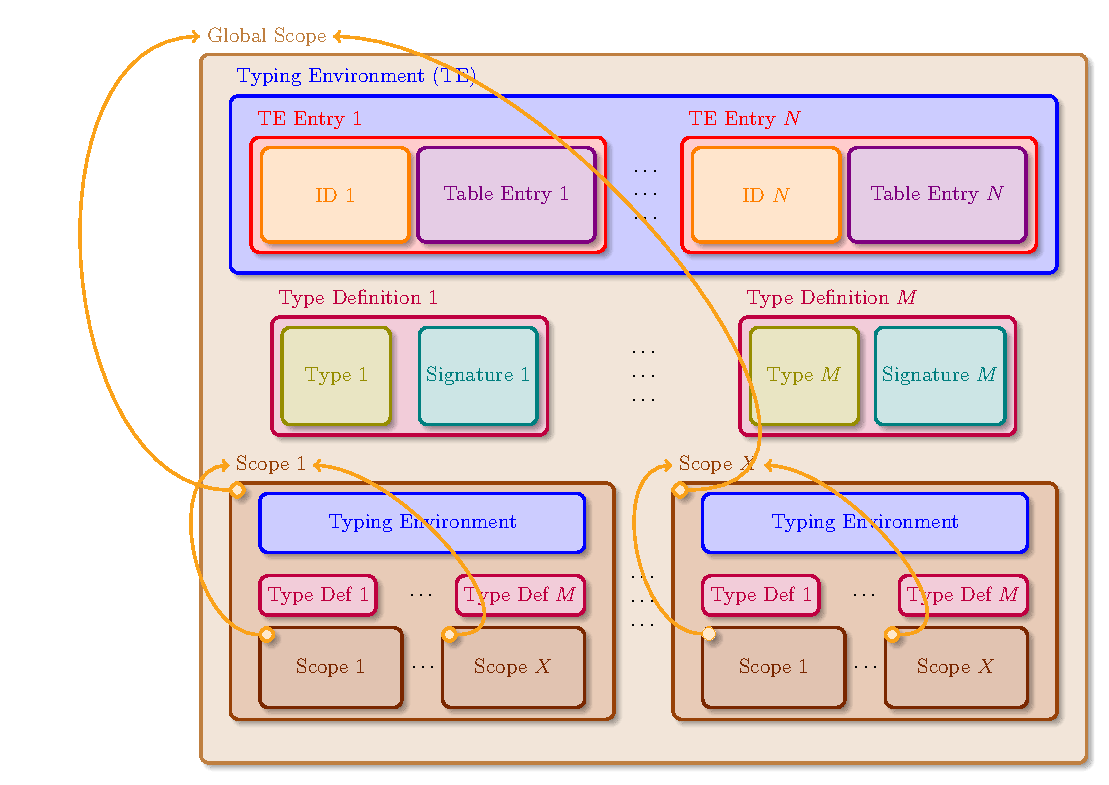
\includegraphics[width=0.9\linewidth]{figs/concept/type_system.pdf}
    \caption{A final representation of the type system}
    \label{lst:concept:type_system}
\end{figure}

\subsection{Example: a simple C program}\label{subsec:concept:ExampleASimpleCProgram}

Now, we propose an example where putting all the concepts together. In Listing~\ref{lst:concept:Example}, we have a simple C program that defines a global variable \texttt{const\_one} and a function \texttt{main} that prints (using the \texttt{printf} function) the value of the variable \texttt{const\_one} and the value of the variable \texttt{two}.

\begin{Listing}[tbh]
    \centering
    \showc*[0.75\textwidth]{Example.c}
    \caption{Example of a simple C program}
    \label{lst:concept:Example}
\end{Listing}

After parsing the program, the \textbf{Typing Environment} should contain the following information:

\begin{table}[t]
    \rowcolors{2}{gray!25}{white}
    % \setlength\arrayrulewidth{0pt}
    \centering
    \begin{tabular}{ c c c c c c }
        \toprule  \textbf{Scope} & \textbf{Identifier} & \textbf{Type} & \textbf{Kind} & \textbf{Location} & \textbf{Details} \\
        \midrule
        \textbf{Global} & \texttt{stdio.h} & \texttt{header} & \texttt{import} & \texttt{1:1 - 1:18} &  \\
        \textbf{Global} & \texttt{const\_one} & \texttt{int} & \texttt{declaration} & \texttt{3:11 - 3:19} & \texttt{const} \\
        \textbf{Global} & \texttt{main} & \texttt{function} & \texttt{declaration} & \texttt{5:5 - 5:8} &  \\
        \textbf{main} & \texttt{two} & \texttt{int} & \texttt{declaration} & \texttt{6:9 - 6:11} & \\
        \textbf{main} & \texttt{printf} & \texttt{function} & \texttt{use} & \texttt{7:5 - 7:10} & \texttt{external} \\
        \textbf{main} & \texttt{const\_one} & \texttt{int} & \texttt{use} & \texttt{7:25 - 7:33} &  \\
        \textbf{main} & \texttt{+} & \texttt{function} & \texttt{use} & \texttt{7:35 - 7:35} &  \\
        \textbf{main} & \texttt{two} & \texttt{int} & \texttt{use} & \texttt{7:37 - 7:39} &  \\
        \bottomrule
    \end{tabular}
    \caption{Language Workbenches Supporting Modularization, Composition and Precompiled Features}
    \label{tab:concept:Example}
\end{table}

\begin{itemize}
    \item The \texttt{stdio.h} header is imported in the \textbf{Global Scope}.
    \item The \texttt{const\_one} variable is declared in the \textbf{Global Scope} as a constant integer.
    \item The \texttt{main} function is declared in the \textbf{Global Scope}.
    \item The \texttt{two} variable is declared in the \texttt{main Scope} as an integer.
    \item The \texttt{printf} function is used in the \texttt{main Scope} and is marked as external.
    \item The \texttt{const\_one} variable is used in the \texttt{main Scope}.
    \item The \texttt{+} operator is used in the \texttt{main Scope}.
    \item The \texttt{two} variable is used in the \texttt{main Scope}.
\end{itemize}

Note that in table~\ref{tab:concept:Example}, we have the \textbf{Scope} as first column, but in reality, is the \textbf{Scope} that defines the visibility and the lifetime of the types in the \textbf{Typing Environment}. In fact, in our explanation in section~\ref{subsec:concept:ScopeTheContextOfTheType}, we defined the \textbf{Scope} as the context in which an identifier is defined, more precisely, where the binding between the type and an identifier is defined in the \textbf{Type System}. So, ideally, every \textbf{Scope} should have a \textbf{Typing Environment} associated with it.
As we can see, these information will be used also to perform the \textbf{modularization} of the LSP (see section~\ref{sec:concept:TowardsAModularTypeSystem}).


\section{Towards a modular type system}\label{sec:concept:TowardsAModularTypeSystem}

In this section, we will discuss the importance of having a modular type system. In particular, we will focus on the ability to define types and operations on these types in a modular way and the ability to combine them.
In the context of language workbenches, the ability to define types and operations on these types in a modular way is crucial. In fact, the language workbenches should be able to support different languages and paradigms, and the ability to define types and operations on these types in a modular way is crucial to achieve this goal.

The \textbf{modularization} of the type system is important for several reasons:
\begin{itemize}
    \item \textbf{Reusability}: The ability to define types and operations on these types in a modular way allows to reuse the types and operations in different contexts.
    \item \textbf{Extensibility}: The ability to define types and operations on these types in a modular way allows to extend the types and operations with new types and operations.
    \item \textbf{Flexibility}: The ability to define types and operations on these types in a modular way allows to adapt the types and operations to the specific needs.
\end{itemize}

In the context of language workbenches and Language Product Lines (SPLs), we are trying to aswer to the following research questions:
\begin{itemize}
    \item[RQ1] How can we define types and operations on these types in a modular way?
    \item[RQ2] How can we combine types and operations on these types in a modular way?
    \item[RQ3] Can we achieve the type checking and type inference in a modular way?
\end{itemize}

\bfcomment{TODO}
Possiamo disabilitare per uno specifico tipo il type checking e il type inference
Dato un linguaggio possiamo avere diversi sistemi di tipi per questo linguaggio
Parliamo di famiglia di sistemi di tipi

\section{The relevance of the type system in the LSP design}\label{sec:concept:RelevanceOfTheTypeSystem}

The type system is the core of the LSP design. We illustrate the need of having a type system by focusing on the ability to respond to requests from a \textit{Language Client}.

In the reminder of this section, we will evaulate the relevance for three of the most important LSP feautre introduced in \ref{subsec:bacground:KeyMethodsOverview}.

\subsubsection{Diagnostic Analysis}\label{subsubsec:concept:DiagnosticAnalysis}

Currently, the LSP provides the ability to perform \textit{diagnostic analysis} on the code. This feature is useful to provide feedback to the user about the correctness of the code.
In compilers design, a \textit{Diagnostic} can be produced by different phases of compilation, such as the \textit{lexical analysis}, \textit{syntax analysis}, and \textit{semantic analysis}.
The \textbf{Syntax Errors} are detected by the \textit{lexical analysis} and \textit{syntax analysis}, usually during the \textit{parsing} phase. The \textbf{Semantic Errors} are detected by the \textit{semantic analysis}, usually during the \textit{type checking} phase.
In modern compilers, an additional phases can be added to the compilation process, \textit{data flow analysis} and \textit{control flow analysis}, that can be used to detect more complex errors, such as \textit{unreachable code} or \textit{dead code}.

In Language Workbenches world, usually it is common to have an instance of a \textbf{Language} and a \textbf{Source Code} that should be parsed and analyzed by the Language.
Taking into account the \textbf{Syntax Errors}, assuming that the \textbf{Language} is able to parse the \textbf{Source Code} and the \textbf{Language} is able to provide errors and warnings during the \textit{parsing} phase, should be easy to provide the \textit{Syntax Errors} to the \textit{Language Client} (see Listing \ref{lst:concept:SyntaxError}).

\begin{Listing}[t]
    \centering
    \showjava*[1\textwidth]{SyntaxError.java}
    \caption{Example of catching a Syntax Error in Java}
    \label{lst:concept:SyntaxError}
\end{Listing}

The \textbf{Semantic Errors} and \textbf{Data Flow Analysis} are more complex to implement. In fact, in order to detect a \textit{Semantic Error}, the \textbf{Language} should be able to perform \textit{type checking} on the \textbf{Source Code} in order to verify that the code can be executed without any unexpected errors. The \textit{Data Flow Analysis} is necessary to understand if the code is reachable, and to do this, the \textbf{Language} should be able to perform static analysis on the \textbf{Source Code}.

\subsubsection{Jump to Definition}\label{subsubsec:concept:JumpToDefinition}
The ability to access the definition of a symbol, such as a function or a variable, is a common feature in modern IDEs.
To enable this functionality, a \textbf{Symbol Table} is required and should be able to map a given row and column position in the source code to the corresponding symbol and its definition.
During this phase, the typechecking is required to bind the symbol to its type. This is necessary to provide the correct definition of the symbol to the user.
In addition to the symbol table, the \textbf{Language} should be able to provide the \textit{Scope} of the symbol, in order to understand if the symbol is visible in the current context.

\subsubsection{Code Completion}\label{subsubsec:concept:CodeCompletion}

To effectively handle this kind of request, such as the one depicted in figure~\ref{fig:completion}, the language server needs to comprehend the type of symbol for which suggestions are to be provided. Once the type is determined, returning relevant suggestions becomes straightforward. However, a challenge arises when suggestions must be presented to the user while they are still writing, as the source code may be syntactically incorrect during the writing process. To address this issue, a parser with error detection and recovery~\cite{Graham79} capabilities is required to enable effective suggestion generation despite the presence of syntax errors.


\section{LSP: a modular approach}\label{sec:concept:LSPAModularApproach}

LSP and DAP are protocols that describes a common \textit{Application Programming Interface} (API) that the \textbf{language server} (LS) should implement, with the benefit of having only one implementation of the LS and multiple clients (IDEs and SCEs) that can consume it, essentially establishing a \textit{client-server} relationship through a communication channel (e.g., \textit{pipes} or \textit{sockets}).
However, the implementation of an LS and its integration with an IDE/SCEs is still a complex task, as it requires the knowledge of the LSP specification and the implementation of the language support.
The implementation~\cite{Gunasinghe22} of an LS is done entirely manually and it is a \textit{top-down} activity, where most of the time is spent on the design and implementation data structures and algorithms.
Since 1990s~\cite{Kang90}, researchers have started talking about the \textit{Software Product Lines} (SPLs) \cite{Cazzola23d, Cazzola20} to move towards a more modular world, where the implementation of a software system can be done in a compositional way, by composing the features of the SPL.
When a SPL is applied to the implementation of a programming language, each product corresponds to a language variant \cite{Cazzola15f} taking the name of \textit{Language Product Lines} (LPLs) \cite{Cazzola15f}. LPLs have been successfully used in both GPLs \cite{Cazzola16, Cazzola16i, Cazzola15f} and DSLs \cite{Haugen08, Cazzola14e, White09}.

\begin{figure}[t]
    \centering
    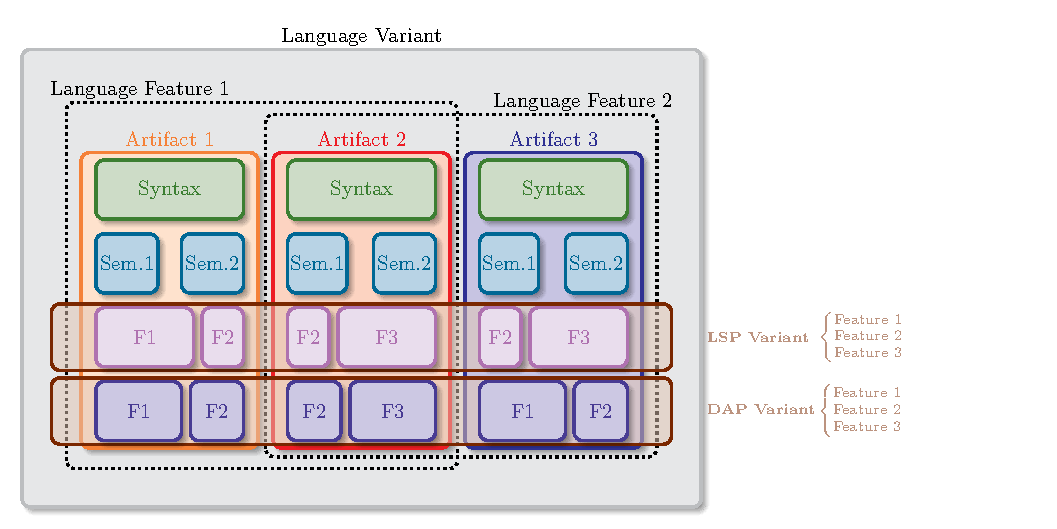
\includegraphics[width=0.9\linewidth]{figs/concept/module_with_lsp.pdf}
    \caption{Proposed approach to modular implementation of LSP and DAP.}
    \label{lst:concept:module_with_lsp}
\end{figure}

What I want to prove with this thesis is that the implementation of an LS could be a \textit{bottom-up} activity, where each LSP or DAP functionality can be seen as a separate \textit{feature module} \cite{Batory04, Kastner11} splitted across the language artifacts, where each artifacts can be part of one or more \textit{language features} (see Figure~\ref{lst:concept:module_with_lsp}). These units can be composed to provide a modular implementation of the LS. This approach is supported by the fact that the LSP and the DAP are \textit{language-agnostic} protocols~\cite{Niephaus20, Rodriguez-Echeverria18} (see Fig.~\ref{lst:lsp}), which means that it does not impose any restrictions on the implementation of the LS, as long as it respects the specification of the protocol.
In \textit{feature-oriented programming} (FOP) \cite{Apel13, Czarnecki04, Prehofer01}, a feature module is a unit of composition that encapsulates a specific functionality, and it is a first-class entity that can be composed with other feature modules to form a software system; similar to an aspect module that encapsulates a crosscutting concern in \textit{aspect-oriented programming} \cite{Kiczales01, Kiczales97, Laddad03}. Using FOP in language development, a family of languages~\cite{Liebig13} can be defined by composing feature modules~\cite{Wende09}, and a language can be seen as a product of the family.
In this way, the implementation of the LS is a \textit{bottom-up} activity, where each artifact has attached a part of LSP and DAP feature module that implements the LS functionality for that \textit{language fragment}, and these units can be composed to provide a modular implementation having \textbf{variants} of the LS.


\section{A \textit{modular} DSL for semplifying the LSP and type system development}\label{sec:concept:AModularDSLForSemplifyingTheLSPAndTypeSystemDevelopment}

\section{Reduce to $\mathcal{L} \times 1$ the number of combinations to support $\mathcal{L}$ languages}

% \begin{figure}[t]
%     \centering
%     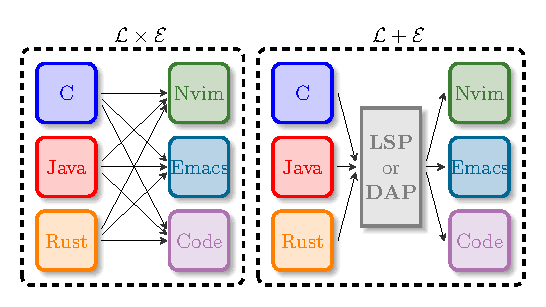
\includegraphics[width=0.9\linewidth]{figs/concept/lsp_combinations.pdf}
%     \caption{Traditional approach vs LSP/DAP approach to language support.}
%     \label{lst:conept:lsp_combinations}
% \end{figure}

